\chapter{Implementacija i korisničko sučelje}
		
		
		\section{Korištene tehnologije i alati}
		
			 {Za komunikaciju unutar tima koristili smo \textbf{Whatsapp}\footnote{\url{https://www.whatsapp.com/}} i \textbf{Discord}\footnote{\url{https://discord.com/}}. Za izradu UML dijagrama koristili smo: \textbf{dbdiagram}\footnote{\url{https://dbdiagram.io/}} za dijagram baze podataka, \textbf{Visual Paradigm Online}\footnote{\url{https://online.visual-paradigm.com/}} za dijagram razreda te \textbf{Astah}\footnote{\url{https://astah.net/}} za ostale UML dijagrame. Kao sustav upravljanja verzijama je korišten \textbf{Git}\footnote{\url{https://git-scm.com/}} te su naši repozitoriji bili dostupni na \textbf{Githubu}\footnote{\url{https://github.com/}} udaljenom repozitoriju.
			 	
		 	Kao razvojno okruženje je korišten \textbf{PyCharm}\footnote{\url{https://www.jetbrains.com/pycharm/}} za razvoj API-ja te \textbf{Android Studio}\footnote{\url{https://developer.android.com/studio}} za razvoj mobilne aplikacije. Pycharm je razvojno okruženje za python, napravljeno od JetBrains-a te Android Studio je modificirana inačica drugog JetBrains razvojnog okruženja (IntelliJ, razvojno okruženje za Javu), prilagođena razvoju android mobilnih aplikacija.
		 	
		 	Mobilna aplikacija je napravljena s pomoću \textbf{Flutter}\footnote{\url{https://flutter.dev/}} razvojnog okvira koji koristi \textbf{Dart}\footnote{\url{https://dart.dev/}} programski jezik. Flutter i Dart su projekti razvijeni od strane Googlea. Flutter je razvojni okvir za izradu aplikacija na različitim platformama, vrlo popularan zbog mogućnosti kreiranja aplikacije za više platforma paralelno. Dart je moderni programski jezik koji se primarno koristi za razvoj Flutter aplikacija.
		 	API je kreiran s pomoću \textbf{Pythona}\footnote{\url{https://www.python.org/}} te \textbf{FastAPI}\footnote{\url{https://fastapi.tiangolo.com/}} razvojnog okvira. FastAPI je novije razvojno okruženje bazirano na Flasku, vrlo popularnom python razvojnom okruženju, s mogućnosti paralelnog izvođenja zahtjeva te automatskom dokumentacijom po OpenAPI standardu.
		 	
		 	Aplikacija je puštena u pogon na \textbf{Renderu}\footnote{\url{https://render.com/}}, te je korišten \textbf{Microsoft Azure}\footnote{\url{https://azure.microsoft.com/}}.
	 	 	za spremanje slika, za prepoznavanje teksta na slikama te se tamo nalazi naša baza podataka.
			 }
			 		
			\eject 
		
	
		\section{Ispitivanje programskog rješenja}
			
			\textbf{\textit{dio 2. revizije}}\\
			
			 \textit{U ovom poglavlju je potrebno opisati provedbu ispitivanja implementiranih funkcionalnosti na razini komponenti i na razini cijelog sustava s prikazom odabranih ispitnih slučajeva. Studenti trebaju ispitati temeljnu funkcionalnost i rubne uvjete.}
	
			
			\subsection{Ispitivanje komponenti}
			%\textit{Potrebno je provesti ispitivanje jedinica (engl. unit testing) nad razredima koji implementiraju temeljne funkcionalnosti. Razraditi \textbf{minimalno 6 ispitnih slučajeva} u kojima će se ispitati redovni slučajevi, rubni uvjeti te izazivanje pogreške (engl. exception throwing). Poželjno je stvoriti i ispitni slučaj koji koristi funkcionalnosti koje nisu implementirane. Potrebno je priložiti izvorni kôd svih ispitnih slučajeva te prikaz rezultata izvođenja ispita u razvojnom okruženju (prolaz/pad ispita). }
			
			{Ispitivanje funkcionalnosti sustava provedeno je uz pomoć unit testova. Testirani su service razredi te pripadajući routeri. U nastavku je priloženo nekoliko primjera tih testova te prikaz rezultata testiranja u razvojnom okruženju.\newline}
			
			{Test za razred UserService kojim se testira ispravno kreiranje novog korisnika. Servisu se šalje objekt tipa UserCreate te u slučaju da direktor još ne postoji očekujemo da će povratna vrijednost biti objekt User s podacima o novom korisniku.}
			
\begin{lstlisting}[style=pythonstyle]
	user_create = UserCreate(email="mail@mail.com",	first_name="Test", last_name="Test", username="test", password="test", roles=[RolesEnum.ADMIN],)
	user = User(id=1, email="test@email.com", first_name="Test", last_name="Test", username="test", roles=[],)
	
	def test_register_user():
		mock_user_crud = Mock()
		mock_user_crud.create_user.return_value = user.model_dump()
		mock_user_crud.get_users_by_role.return_value = None
		db = Mock()
		
		user_service = UserService(db)
		
		with patch("app.services.users.UserCRUD", 
					return_value=mock_user_crud):
			result = user_service.register_user(user_create)
		
		mock_user_crud.create_user.assert_called_once_with(user_create)
		mock_user_crud.get_users_by_role.assert_not_called()
		assert result == user.model_dump()
\end{lstlisting}
			
			{Sljedećim testom za documents router testira se reakcija pokušaja dohvaćanja povijesti skeniranih dokumenata za korisnika koji nije ulogiran te se očekuje 'NotAuthenticated' iznimka od servera.}
			
\begin{lstlisting}[style=pythonstyle]
	def test_get_me_not_authenticated():
		response = client.get("/documents/me")
		assert response.status_code == 401
		assert response.json() == {'app_exception': 'NotAuthenticated', 'context': {}}
\end{lstlisting}

			{Test za razred DocumentService koji testira kreiranje dokumenta. Servisu šaljemo sliku i korisničko ime te ako je dokument uspješno kreiran očekujemo da će nam servis vratiti kreirani novi objekt tipa Document sa svim podacima o dokumentu.}
			
\begin{lstlisting}[style=pythonstyle]
	@patch("app.services.documents.detect_document", return_value="R123456 text")
	def test_create_document(detect_document):
		mock_document_crud = Mock()
		mock_document_crud.create_document.return_value = document1
		
		mock_user_service = Mock()
		mock_user_service.get_user.return_value = admin
		
		mock_image_service = Mock()
		mock_image_service.create_image.return_value = imageDB
		db = Mock()
		
		document_service = DocumentService(db)
		
		with patch("app.services.documents.DocumentCRUD", return_value=mock_document_crud), patch("app.services.documents.ImageService", return_value=mock_image_service), patch("app.services.documents.UserService", return_value=mock_user_service):
			result = document_service.create_document(uploaded_image, "username")
		
		detect_document.assert_called_once()
		mock_user_service.get_user.assert_called_once()
		mock_image_service.create_image.assert_called_once()
		
		assert result == document1
\end{lstlisting}

			{Sljedeća dva testa testiraju ažuriranje statusa dokumenta u razredu DocumentService. Prvi provjerava dozvoljeni slučaj iz APPROVED želimo status postaviti na AUDITED, stoga nakon što servisu pošaljemo id dokumenta novi status te eventualne promjene u samom tekstualnom sadržaju očekujemo da će nam vratiti taj dokument s novim statusom. Drugi provjerava slučaj u kojem smo nakon statusa APPROVED odmah skočili na status ARCHIVED. Budući da to nije dozvoljeni slijed statusa očekujemo da će nam servis baciti iznimku "DocumentException.DocumentStatusNotCompatible".}
			
\begin{lstlisting}[style=pythonstyle]
	document2 = Document(id=2, image_id=1, owner=director, document_type=DocumentTypeEnum.INTERNAL, summary="test", document_status=DocumentStatusEnum.APPROVED, scan_time="2021-01-01T00:00:00",)
	document3 = Document(id=2, image_id=1, owner=director, document_type=DocumentTypeEnum.INTERNAL, summary="test", document_status=DocumentStatusEnum.AUDITED, scan_time="2021-01-01T00:00:00",)	

	def test_update_document():
		mock_document_crud = Mock(spec=DocumentCRUD)
		mock_document = Mock(spec=document2, document_status=DocumentStatusEnum.APPROVED)
		mock_document_crud.get_document.return_value = mock_document
		mock_document_crud.update_document.return_value = document3
		db = Mock()
		
		document_service = DocumentService(db)
		
		with patch("app.services.documents.DocumentCRUD", return_value=mock_document_crud):
		result = document_service.update_document(2, DocumentStatusEnum.AUDITED, None)
		
		mock_document_crud.update_document.assert_called_once()
		assert result == document3
	
	def test_update_document_with_invalid_status():
		mock_document_crud = Mock(spec=DocumentCRUD)
		mock_document = Mock(spec=document2, document_status=DocumentStatusEnum.APPROVED)
		mock_document_crud.get_document.return_value = mock_document
		mock_document_crud.update_document.return_value = document3
		db = Mock()
		
		document_service = DocumentService(db)
		
		with patch("app.services.documents.DocumentCRUD", return_value=mock_document_crud):
		with raises(DocumentException.DocumentStatusNotCompatible):
		document_service.update_document(2, DocumentStatusEnum.ARCHIVED, None)
\end{lstlisting}

			{Posljednji testovi testiraju arhiviranje dokumenta u sklopu ArchiveService-a. Dokument se smije arhivirati ako je prethodni status bio PENDING ili SIGNED\textunderscore PENDING. U prvom testu želimo arhivirati dokument čiji status arhiviranja je PENDING te ga želimo postaviti na DONE što je dozvoljeni slijed statusa. Očekuje se uspješni završetak metode archive\textunderscore document koja onda vraća arhivirani dokument s novim statusom DONE.
			U drugom testu želimo isprobati slučaj u kojem pokušavamo dokument iz AWAITING\textunderscore SIGNATURE statusa pretvoriti u DONE što nije dopušteni slijed stanja pa je i očekivano bacanje iznimke "ArchiveException.IllegalArchiveStatus".}
			
\begin{lstlisting}[style=pythonstyle]
	def test_archive_document():
		mock_archive_crud = Mock()
		mock_archive_crud.get_archived_by_document_id.return_value = archive1
		mock_archive_crud.update_archive.return_value = archive1
		
		mock_user_service = Mock(spec=UserService)
		mock_user_service.get_user.return_value = admin
		
		mock_document_service = Mock(spec=DocumentService)
		mock_document_service.update_document.return_value = None
		
		db = Mock()
		
		archive_service = ArchiveService(db)
		
		with patch("app.services.archives.ArchiveCRUD", return_value=mock_archive_crud):
			with patch("app.services.archives.UserService", return_value=mock_user_service):
				with patch("app.services.archives.DocumentService", return_value=mock_document_service):
					result = archive_service.archive_document(1, ArchiveStatus.DONE, "test")
		
		mock_archive_crud.get_archived_by_document_id.assert_called_once_with(1)
		mock_archive_crud.update_archive.assert_called_once()
		assert result == archive1
		
	def test_archive_document_forbidden():
		mock_archive_crud = Mock()
		mock_archive_crud.get_archived_by_document_id.return_value = archive3
		mock_archive_crud.update_archive.return_value = archive1
		
		mock_user_service = Mock(spec=UserService)
		mock_user_service.get_user.return_value = admin
		
		mock_document_service = Mock(spec=DocumentService)
		mock_document_service.update_document.return_value = None
		
		db = Mock()
		
		archive_service = ArchiveService(db)
		
		with patch("app.services.archives.ArchiveCRUD", 	return_value=mock_archive_crud):
			with patch("app.services.archives.UserService", return_value=mock_user_service):
				with patch("app.services.archives.DocumentService", return_value=mock_document_service):
					with raises(ArchiveException.IllegalArchiveStatus):
						archive_service.archive_document(1, ArchiveStatus.DONE, "test")
\end{lstlisting}

			{Svi navedeni ispitni slučajevi prošli su testiranje.}

			\begin{figure}[H]
				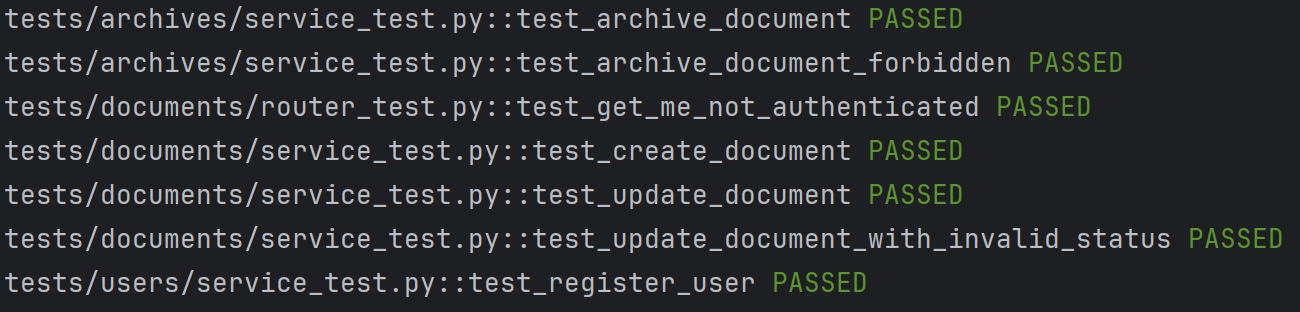
\includegraphics[width=\textwidth]{slike/unitTestovi.png}
				\caption{Prikaz rezultata ispitnih slučajeva u razvojnom okruženju}
				\label{fig:rezultatiUnitTestova}
			\end{figure}		
			
			
			\subsection{Ispitivanje sustava}
			
			 {Razvojni okvir Flutter pruža niz službenih, integriranih alata za izvršavanje više vrsta testova. Ovisno o razini ili dijelu sustava koji se testira dostupni testovi unutar Flutter paketa su Unit, Widget i Integration testovi. Unutar Flutter okvira Integration testovi služe za testiranje čitavog ili pojedinih dijelova sustav, odnosno preuzimaju ulogu integracijskih i sustavnih testova ovisno o implementaciji, a pišu se unutar samog projekta s pomoću jezika Dart, što olakšava održavanje. Integrirani paketi također pružaju mogućnost automatizacije testova, simulacije i praćenja korisničkih unosa, praćenje tijeka izvođenja i mrežnog prometa na simuliranim i stvarnim uređajima te lakog pregleda uspješnosti i ispisa provedenih testova. Iz navedenih razloga za testiranje aplikacije korišteni su integrirani alati dostupni unutar paketa flutter\_test i integration\_test. Druga mogućnost bila bi uporaba Appium alata koji se temelji na Selenium strukturi. Dostupni su preko javno održavanih paketa za prilagodbu, no integrirani alati pokazuju se boljim rješenjem za dani slučaj.}
			 
			 {U nastavku su opisani izvedeni testovi sustava. Tijelo svakog testa se sastoji od grupa, a tijelo svake grupe od podtestova. Sve grupe i podtestovi se vrše slijedno, sukladno hijerarhiji definiranoj u implementaciji te predstavljaju korake i potkorake u testiranju. Cilj sljedećih testova je utvrditi ispunjava li potpuno integrirani sustav zadaće u konkretnim slučajevima i prilagođava li se mogućim rubnim slučajevima. Također se želi sagledati mogu li se svi testovi izvršiti slijedno čime se utvrđuje stabilnost sustava. Za svaki testni slučaj opisani su ulazni podaci i početno stanje, koraci testa, očekivani i stvarni rezultat te ocjena rezultata i tijeka izvođenja. Testovi se izvode u trenutku kad postoji konkretna količina podataka za testiranje kao i sve vrste potrebnih korisnika.}
			 
			 \subsubsection{Test uspješne i neuspješne prijave te odjave}
			 
			 \begin{itemize}
			 	
			 \item{\textbf{Ulazni podaci:}}
			 \begin{itemize}
			 	\item{username1: admin}
			 	\item{password1: admin}
			 	\item{username2: admin}
			 	\item{password2: neadmin}
			 \end{itemize}
			 
			 \item{\textbf{Početno stanje:} Aplikacija u početnom stanju bez prijavljenog korisnika.}
			 
			 \item{\textbf{Koraci testa:} Koraci koji se provode u testu jesu; upisivanje prvih ulaznih podataka u formular za prijavu i pritisak na gumb za prijavu, navigacija na home screen, otvaranje sučelja za navigaciju i pritisak na gumb za odjavu, upisivanje drugih ulaznih podatak u formular za prijavu i pritisak na gumb za prijavu.}
			 
			 \item{\textbf{Očekivani rezultat:} Očekuje se navigacija na home screen nakon upisa valjanih podataka za prijavu, pravilno otvaranje sučelja za navigaciju, povratak na login screen te ostanak na istom nakon upisa nevaljanih podataka.}
			 
			 \item{\textbf{Stvarni rezultat:} Provedeni koraci se poklapaju s očekivanim, test prolazi.}
			 
			 \item{\textbf{Ocjena:} Testirane funkcionalnosti su zadovoljavajuće, rade ispravno, no može se primijetiti nedostatak povratnih informacija pri neuspješnom prijavljivanju zbog neimplementiranih funkcionalnosti.}
			 
			\end{itemize}
			
			\subsubsection{Test pregleda korisnika}
			
			\begin{itemize}
				
				\item{\textbf{Ulazni podaci:}}
				\begin{itemize}
					\item{username: owner}
					\item{password: owner}
				\end{itemize}
				
				\item{\textbf{Početno stanje:} Nastavak nakon prethodnog testa, bez prijavljenog korisnika (reset sa zastavicom.}
				
				\item{\textbf{Koraci testa:} Koraci koji se provode u testu jesu; upisivanje ulaznih podataka u formular za prijavu i pritisak na gumb za prijavu, navigacija na home screen, otvaranje sučelja za navigaciju i navigacija na users screen (Korisnici), ako se pronađe korisnik pritisak na gumb za statistiku, nakon otvaranja pritisak na gumb za zatvaranje dijaloga.}
				
				\item{\textbf{Očekivani rezultat:} Očekuje se navigacija na home screen nakon upisa valjanih podataka za prijavu, pravilno otvaranje sučelja za navigaciju, navigacija na users screen, ako se pronađe korisnik uspješno otvaranje dijaloga za pregled statistike te uspješno zatvaranje dijaloga i ostanaka na users screen.}
				
				\item{\textbf{Stvarni rezultat:} Provedeni koraci se poklapaju s očekivanim, test prolazi.}
				
				\item{\textbf{Ocjena:} Testirane funkcionalnosti su zadovoljavajuće, rade ispravno.}
				
			\end{itemize}
			
			\subsubsection{Test pregleda dokumenata}
			
			\begin{itemize}
				
				\item{\textbf{Ulazni podaci:}}
				\begin{itemize}
					\item{username: owner}
					\item{password: owner}
				\end{itemize}
				
				\item{\textbf{Početno stanje:} Nastavak nakon prethodnog testa, bez prijavljenog korisnika (reset sa zastavicom).}
				
				\item{\textbf{Koraci testa:} Koraci koji se provode u testu jesu; upisivanje ulaznih podataka u formular za prijavu i pritisak na gumb za prijavu, navigacija na home screen, otvaranje sučelja za navigaciju i navigacija na documents screen (Povijest), ako se pronađe dokument pritisak na gumb za pregled PDF dokumenta i navigacija na sučelje za pregled, simulacija izlaska iz sučelja.}
				
				\item{\textbf{Očekivani rezultat:} Očekuje se navigacija na home screen nakon upisa valjanih podataka za prijavu, pravilno otvaranje sučelja za navigaciju, navigacija na documents screen (Povijest), ako se pronađe dokument uspješno otvaranje sučelja za pregled PDF dokumenta te uspješan povratak na pregled, u suprotnom ostanak na documents screen.}
				
				\item{\textbf{Stvarni rezultat:} Provedeni koraci se poklapaju s očekivanim, test prolazi.}
				
				\item{\textbf{Ocjena:} Testirane funkcionalnosti su zadovoljavajuće, rade ispravno.}
				
			\end{itemize}
			
			\subsubsection{Test revizije dokumenata}
			
			\begin{itemize}
				
				\item{\textbf{Ulazni podaci:}}
				\begin{itemize}
					\item{username: revizor1}
					\item{password: revizor1}
				\end{itemize}
				
				\item{\textbf{Početno stanje:} Nastavak nakon prethodnog testa, bez prijavljenog korisnika (reset sa zastavicom).}
				
				\item{\textbf{Koraci testa:} Koraci koji se provode u testu jesu; upisivanje ulaznih podataka u formular za prijavu i pritisak na gumb za prijavu, navigacija na home screen, otvaranje sučelja za navigaciju i navigacija na revision screen (Revizije), ako se pronađe dokument pritisak na gumb za revidiranje i navigacija na sučelje za revidiranje, pritisak na gumb za revidiranje, otvaranje dijaloga za uspješnu reviziju, pritisak na gumb za zatvaranje dijaloga i povratak na revision screen, događa se reset, ponavljaju se koraci za navigaciju na revision screen, pritisak na tab za revidirane dokumente (Revidirani).}
				
				\item{\textbf{Očekivani rezultat:} Očekuje se navigacija na home screen nakon upisa valjanih podataka za prijavu, pravilno otvaranje sučelja za navigaciju, navigacija na revision screen (Revizije), ako se pronađe dokument uspješno otvaranje sučelja za revidiranje, uspješno revidiranje i otvaranje povezanog dijaloga, zatvaranje dijaloga i izlazak na revision screen, nakon reseta uspješan povratak na revision screen i uspješno otvaranje taba za pregled revidiranih dokumenata.}
				
				\item{\textbf{Stvarni rezultat:} Provedeni koraci se poklapaju s očekivanim, test prolazi.}
				
				\item{\textbf{Ocjena:} Testirane funkcionalnosti su zadovoljavajuće, rade ispravno.}
				
			\end{itemize}
			
			\subsubsection{Test arhiviranja dokumenata}
			
			\begin{itemize}
				
				\item{\textbf{Ulazni podaci:}}
				\begin{itemize}
					\item{username: racunovoda1}
					\item{password: racunovoda1}
				\end{itemize}
				
				\item{\textbf{Početno stanje:} Nastavak nakon prethodnog testa, bez prijavljenog korisnika (reset sa zastavicom).}
				
				\item{\textbf{Koraci testa:} Koraci koji se provode u testu jesu; upisivanje ulaznih podataka u formular za prijavu i pritisak na gumb za prijavu, navigacija na home screen, otvaranje sučelja za navigaciju i navigacija na archive screen (Arhiva), ako se pronađe dokument pritisak na gumb za arhiviranje i navigacija na sučelje za arhiviranje, pritisak na gumb za arhiviranje, otvaranje dijaloga za uspješno arhiviranje, pritisak na gumb za zatvaranje dijaloga i povratak na archive screen, događa se reset, ponavljaju se koraci za navigaciju na archive screen, pritisak na tab za arhivirane dokumente (Arhivirani).}
				
				\item{\textbf{Očekivani rezultat:} Očekuje se navigacija na home screen nakon upisa valjanih podataka za prijavu, pravilno otvaranje sučelja za navigaciju, navigacija na archive screen (Arhiva), ako se pronađe dokument uspješno otvaranje sučelja za arhiviranje, uspješno arhiviranje i otvaranje povezanog dijaloga, zatvaranje dijaloga i izlazak na archive screen, nakon reseta uspješan povratak na archive screen i uspješno otvaranje taba za pregled arhiviranih dokumenata.}
				
				\item{\textbf{Stvarni rezultat:} Provedeni koraci se poklapaju s očekivanim, test prolazi.}
				
				\item{\textbf{Ocjena:} Testirane funkcionalnosti su zadovoljavajuće, rade ispravno.}
				
			\end{itemize}
			
			\subsubsection{Zaključak i osvrt na testiranje sustava}
			
			{Svi testovi uspješno su slijedno provedeni čime se može zaključiti kako su proučene funkcionalnosti skladne i ispravne. Nisu pronađene greške u sučelje koje onemogućuju izvođenje očekivanih nizova akcija. Nisu pronađene greške u pozadinskom baratanju stanja koje bi onemogućilo pravilno izmjenjivanja sesija, što se može zaključiti iz ispravne promjene aktivnih korisnika između testova. Dohvaćanje podataka i komunikacija s poslužiteljem u danim slučajevima također se mogu procijeniti kao ispravni zbog izostanka grešaka.}
				
			{Zamjerke se odnose na moguća poboljšanja sučelja za prijavu gdje ne postoje nikakve povratne informacije u slučaju neispravnih podataka za prijavu. Također se može napomenuti kako trenutna količina testova nije dovoljna za detaljno testiranje sustava te se ne provede testovi za neke ključne funkcionalnosti poput stvaranja korisnika, skeniranja i digitalizacije dokumenata te prosljeđivanja. Glavni razlog ne provođenja veće količine testova je vrijeme, a može se spomenuti i problematika testiranja funkcionalnosti koje se oslanjaju na upotrebljene pakete za čiju provjera bi valjalo detaljnije proučiti implementaciju samih paketa.}
			 
			\eject 
		
		
		\section{Dijagram razmještaja}
			
			\textbf{\textit{dio 2. revizije}}
			
			 \textit{Potrebno je umetnuti \textbf{specifikacijski} dijagram razmještaja i opisati ga. Moguće je umjesto specifikacijskog dijagrama razmještaja umetnuti dijagram razmještaja instanci, pod uvjetom da taj dijagram bolje opisuje neki važniji dio sustava.}
			
			\eject 
		
		\section{Upute za puštanje u pogon}
		
			\textbf{\textit{dio 2. revizije}}\\
		
			 \textit{U ovom poglavlju potrebno je dati upute za puštanje u pogon (engl. deployment) ostvarene aplikacije. Na primjer, za web aplikacije, opisati postupak kojim se od izvornog kôda dolazi do potpuno postavljene baze podataka i poslužitelja koji odgovara na upite korisnika. Za mobilnu aplikaciju, postupak kojim se aplikacija izgradi, te postavi na neku od trgovina. Za stolnu (engl. desktop) aplikaciju, postupak kojim se aplikacija instalira na računalo. Ukoliko mobilne i stolne aplikacije komuniciraju s poslužiteljem i/ili bazom podataka, opisati i postupak njihovog postavljanja. Pri izradi uputa preporučuje se \textbf{naglasiti korake instalacije uporabom natuknica} te koristiti što je više moguće \textbf{slike ekrana} (engl. screenshots) kako bi upute bile jasne i jednostavne za slijediti.}
			
			
			 \textit{Dovršenu aplikaciju potrebno je pokrenuti na javno dostupnom poslužitelju. Studentima se preporuča korištenje neke od sljedećih besplatnih usluga: \href{https://aws.amazon.com/}{Amazon AWS}, \href{https://azure.microsoft.com/en-us/}{Microsoft Azure} ili \href{https://www.heroku.com/}{Heroku}. Mobilne aplikacije trebaju biti objavljene na F-Droid, Google Play ili Amazon App trgovini.}
			
			
			\eject 